\documentclass{ximera}

\title{Practice for Forced Oscillations}

%\auor{Matthew Charnley and Jason Nowell}
\usepackage[margin=1.5cm]{geometry}
\usepackage{indentfirst}
\usepackage{sagetex}
\usepackage{lipsum}
\usepackage{amsmath}
\usepackage{mathrsfs}


%%% Random packages added without verifying what they are really doing - just to get initial compile to work.
\usepackage{tcolorbox}
\usepackage{hypcap}
\usepackage{booktabs}%% To get \toprule,\midrule,\bottomrule etc.
\usepackage{nicefrac}
\usepackage{caption}
\usepackage{units}

% This is my modified wrapfig that doesn't use intextsep
\usepackage{mywrapfig}
\usepackage{import}



%%% End to random added packages.


\graphicspath{
    {./figures/}
    {./../figures/}
    {./../../figures/}
}
\renewcommand{\log}{\ln}%%%%
\DeclareMathOperator{\arcsec}{arcsec}
%% New commands


%%%%%%%%%%%%%%%%%%%%
% New Conditionals %
%%%%%%%%%%%%%%%%%%%%


% referencing
\makeatletter
    \DeclareRobustCommand{\myvref}[2]{%
      \leavevmode%
      \begingroup
        \let\T@pageref\@pagerefstar
        \hyperref[{#2}]{%
	  #1~\ref*{#2}%
        }%
        \vpageref[\unskip]{#2}%
      \endgroup
    }%

    \DeclareRobustCommand{\myref}[2]{%
      \leavevmode%
      \begingroup
        \let\T@pageref\@pagerefstar
        \hyperref[{#2}]{%
	  #1~\ref*{#2}%
        }%
      \endgroup
    }%
\makeatother

\newcommand{\figurevref}[1]{\myvref{Figure}{#1}}
\newcommand{\figureref}[1]{\myref{Figure}{#1}}
\newcommand{\tablevref}[1]{\myvref{Table}{#1}}
\newcommand{\tableref}[1]{\myref{Table}{#1}}
\newcommand{\chapterref}[1]{\myref{chapter}{#1}}
\newcommand{\Chapterref}[1]{\myref{Chapter}{#1}}
\newcommand{\appendixref}[1]{\myref{appendix}{#1}}
\newcommand{\Appendixref}[1]{\myref{Appendix}{#1}}
\newcommand{\sectionref}[1]{\myref{\S}{#1}}
\newcommand{\subsectionref}[1]{\myref{subsection}{#1}}
\newcommand{\subsectionvref}[1]{\myvref{subsection}{#1}}
\newcommand{\exercisevref}[1]{\myvref{Exercise}{#1}}
\newcommand{\exerciseref}[1]{\myref{Exercise}{#1}}
\newcommand{\examplevref}[1]{\myvref{Example}{#1}}
\newcommand{\exampleref}[1]{\myref{Example}{#1}}
\newcommand{\thmvref}[1]{\myvref{Theorem}{#1}}
\newcommand{\thmref}[1]{\myref{Theorem}{#1}}


\renewcommand{\exampleref}[1]{ {\color{red} \bfseries Normally a reference to a previous example goes here.}}
\renewcommand{\figurevref}[1]{ {\color{red} \bfseries Normally a reference to a previous figure goes here.}}
\renewcommand{\tablevref}[1]{ {\color{red} \bfseries Normally a reference to a previous table goes here.}}
\renewcommand{\Appendixref}[1]{ {\color{red} \bfseries Normally a reference to an Appendix goes here.}}
\renewcommand{\exercisevref}[1]{ {\color{red} \bfseries Normally a reference to a previous exercise goes here.}}



\newcommand{\R}{\mathbb{R}}

%% Example Solution Env.
\def\beginSolclaim{\par\addvspace{\medskipamount}\noindent\hbox{\bf Solution:}\hspace{0.5em}\ignorespaces}
\def\endSolclaim{\par\addvspace{-1em}\hfill\rule{1em}{0.4pt}\hspace{-0.4pt}\rule{0.4pt}{1em}\par\addvspace{\medskipamount}}
\newenvironment{exampleSol}[1][]{\beginSolclaim}{\endSolclaim}

%% General figure formating from original book.
\newcommand{\mybeginframe}{%
\begin{tcolorbox}[colback=white,colframe=lightgray,left=5pt,right=5pt]%
}
\newcommand{\myendframe}{%
\end{tcolorbox}%
}

%%% Eventually return and fix this to make matlab code work correctly.
%% Define the matlab environment as another code environment
%\newenvironment{matlab}
%{% Begin Environment Code
%{ \centering \bfseries Matlab Code }
%\begin{code}
%}% End of Begin Environment Code
%{% Start of End Environment Code
%\end{code}
%}% End of End Environment Code


% this one should have a caption, first argument is the size
\newenvironment{mywrapfig}[2][]{
 \wrapfigure[#1]{r}{#2}
 \mybeginframe
 \centering
}{%
 \myendframe
 \endwrapfigure
}

% this one has no caption, first argument is size,
% the second argument is a larger size used for HTML (ignored by latex)
\newenvironment{mywrapfigsimp}[3][]{%
 \wrapfigure[#1]{r}{#2}%
 \centering%
}{%
 \endwrapfigure%
}
\newenvironment{myfig}
    {%
    \begin{figure}[h!t]
        \mybeginframe%
        \centering%
    }
    {%
        \myendframe
    \end{figure}%
    }


% graphics include
\newcommand{\diffyincludegraphics}[3]{\includegraphics[#1]{#3}}
\newcommand{\myincludegraphics}[3]{\includegraphics[#1]{#3}}
\newcommand{\inputpdft}[1]{\subimport*{../figures/}{#1.pdf_t}}


%% Not sure what these even do? They don't seem to actually work... fun!
%\newcommand{\mybxbg}[1]{\tcboxmath[colback=white,colframe=black,boxrule=0.5pt,top=1.5pt,bottom=1.5pt]{#1}}
%\newcommand{\mybxsm}[1]{\tcboxmath[colback=white,colframe=black,boxrule=0.5pt,left=0pt,right=0pt,top=0pt,bottom=0pt]{#1}}
\newcommand{\mybxsm}[1]{#1}
\newcommand{\mybxbg}[1]{#1}

%%% Something about tasks for practice/hw?
\usepackage{tasks}
\usepackage{footnote}
\makesavenoteenv{tasks}


%% For pdf only?
\newcommand{\diffypdfversion}[1]{#1}


%% Kill ``cite'' and go back later to fix it.
\renewcommand{\cite}[1]{}


%% Currently we can't really use index or its derivatives. So we are gonna kill them off.
\renewcommand{\index}[1]{}
\newcommand{\myindex}[1]{#1}







\begin{document}
\begin{abstract}
Why?
\end{abstract}
\maketitle


\begin{exercise}
    On a piece of graph paper draw the vectors:
    \begin{tasks}(3)
        \task
        $\begin{bmatrix}
            2 \\
            5 
        \end{bmatrix}$
        \task
        $\begin{bmatrix}
            -2 \\
            -4
        \end{bmatrix}$
        \task $(3,-4)$
    \end{tasks}
\end{exercise}
%\comboSol
%{%
%a)~\parbox[c]{1.4in}{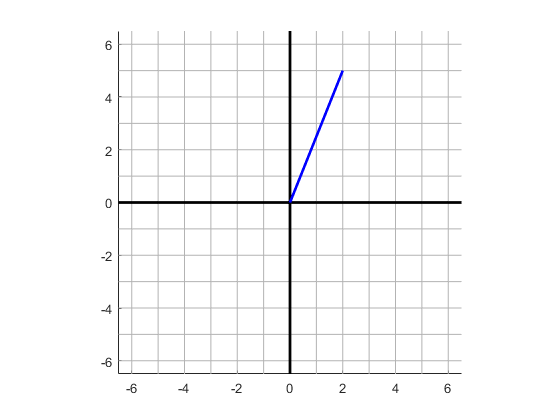
\includegraphics[width=1.4in]{Images/vectorplot25.png}} \quad b)~\parbox[c]{1.4in}{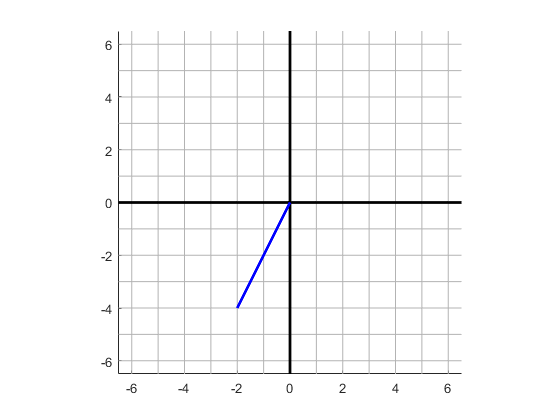
\includegraphics[width=1.4in]{Images/vectorplotm2m4.png}} \quad c)~\parbox[c]{1.4in}{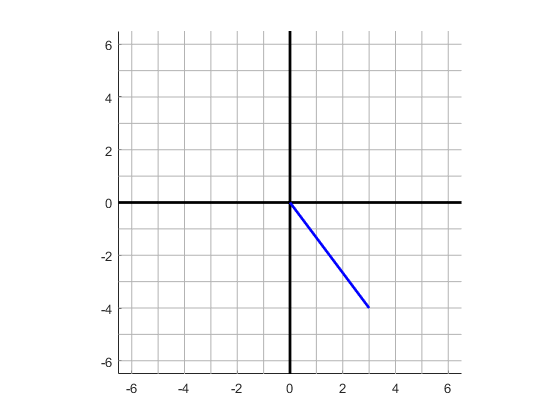
\includegraphics[width=1.4in]{Images/vectorplot3m4.png}}
%}

\begin{exercise}
    On a piece of graph paper draw the vector $(1,2)$ starting at (based at) the given point:
    \begin{tasks}(3)
        \task based at $(0,0)$
        \task based at $(1,2)$
        \task based at $(0,-1)$
    \end{tasks}
\end{exercise}
%\comboSol
%{%
%a)~\parbox[c]{1.4in}{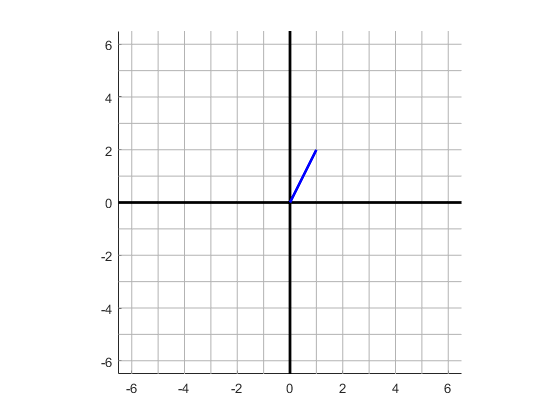
\includegraphics[width=1.4in]{Images/vectorplot1200.png}} \quad b)~\parbox[c]{1.4in}{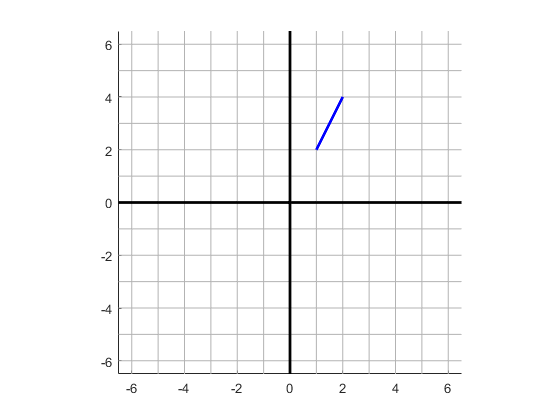
\includegraphics[width=1.4in]{Images/vectorplot1212.png}} \quad c)~\parbox[c]{1.4in}{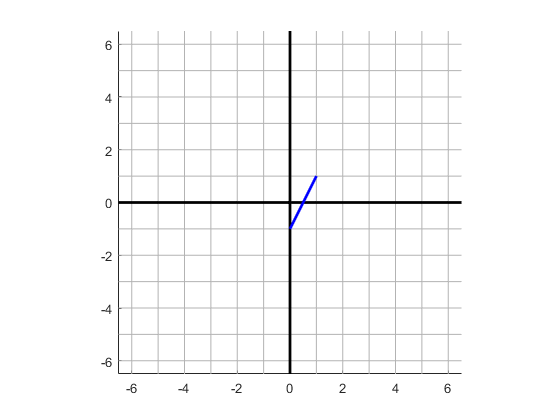
\includegraphics[width=1.4in]{Images/vectorplot120m1.png}}
%}

\begin{exercise}
    On a piece of graph paper draw the following operations.  Draw and label the vectors involved in the operations as well as the result:
    \begin{tasks}(3)
        \task
        $\begin{bmatrix}
            1 \\
            -4
        \end{bmatrix}
        +
        \begin{bmatrix}
            2 \\
            3
        \end{bmatrix}$
        \task
        $\begin{bmatrix}
            -3 \\
            2
        \end{bmatrix}
        -
        \begin{bmatrix}
            1 \\
            3
        \end{bmatrix}$
        \task
        $3\begin{bmatrix}
            2 \\
            1
        \end{bmatrix}$
    \end{tasks}
\end{exercise}
%\comboSol
%{%
%a)~\parbox[c]{1.4in}{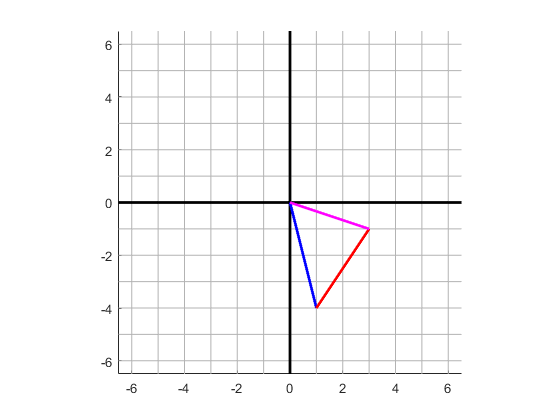
\includegraphics[width=1.4in]{Images/vectorops1.png}} \quad b)~\parbox[c]{1.4in}{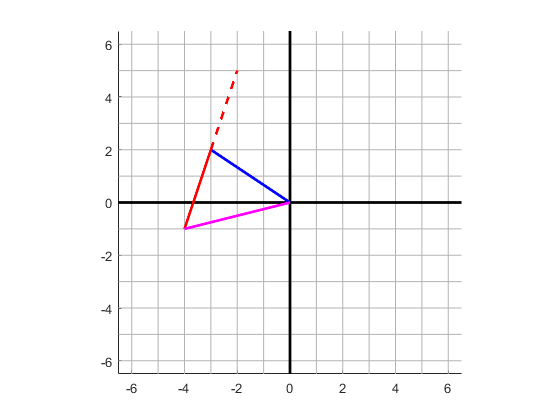
\includegraphics[width=1.4in]{Images/vectorops2.png}} \quad c)~\parbox[c]{1.4in}{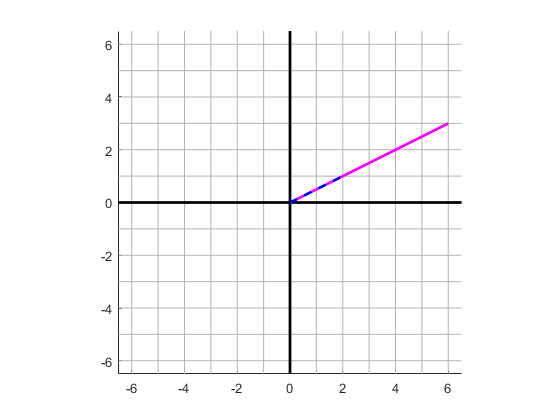
\includegraphics[width=1.4in]{Images/vectorops3.png}}
%}

\begin{exercise}
    Compute the magnitude of
    \begin{tasks}(3)
        \task
        $\begin{bmatrix}
            7 \\
            2 
        \end{bmatrix}$
        \task
        $\begin{bmatrix}
            -2 \\
            3 \\
            1
        \end{bmatrix}$
        \task $(1,3,-4)$
    \end{tasks}
\end{exercise}
%\comboSol
%{%
%a)~ $\sqrt{53}$ \quad b~) $\sqrt{14}$ \quad c)~ $\sqrt{26}$
%}

\begin{exercise}%
    Compute the magnitude of
    \begin{tasks}(3)
        \task
        $\begin{bmatrix}
            1 \\
            3
        \end{bmatrix}$
        \task
        $\begin{bmatrix}
            2 \\
            3 \\
            -1
        \end{bmatrix}$
        \task $(-2,1,-2)$
    \end{tasks}
\end{exercise}
%\exsol{%
%a)~$\sqrt{10}$
%\quad b)~$\sqrt{14}$
%\quad c)~$3$
%}

\begin{exercise}
    Compute
    \begin{tasks}(3)
        \task
        $\begin{bmatrix}
            2 \\
            3 
        \end{bmatrix}
        +
        \begin{bmatrix}
            7 \\
            -8
        \end{bmatrix}$
        \task
        $\begin{bmatrix}
            -2 \\
            3 
        \end{bmatrix}
        -
        \begin{bmatrix}
            6 \\
            -4
        \end{bmatrix}$
        \task
        $-\begin{bmatrix}
            -3 \\
            2 
        \end{bmatrix}$
        \task
        $4\begin{bmatrix}
            -1 \\
            5 
        \end{bmatrix}$
        \task
        $5\begin{bmatrix}
            1 \\
            0 
        \end{bmatrix}
        + 9
        \begin{bmatrix}
            0 \\
            1
        \end{bmatrix}$
        \task
        $3\begin{bmatrix}
            1 \\
            -8 
        \end{bmatrix}
        - 2
        \begin{bmatrix}
            3 \\
            -1
        \end{bmatrix}$
    \end{tasks}
\end{exercise}
%\comboSol
%{%
%a) $\left[\begin{smallmatrix} 9 \\ -5 \end{smallmatrix}\right]$ \quad b)~ $\left[\begin{smallmatrix}  -8 \\ 7 \end{smallmatrix}\right]$ \quad c)~ $\left[\begin{smallmatrix} 3 \\ -2 \end{smallmatrix}\right]$ \quad
%d)~ $\left[\begin{smallmatrix} -4 \\ 20 \end{smallmatrix}\right]$ \quad e)~ $\left[\begin{smallmatrix} 5 \\ 9 \end{smallmatrix}\right]$ \quad f)~ $\left[\begin{smallmatrix} -3 \\ -22 \end{smallmatrix}\right]$
%}

\begin{exercise}%
    Compute
    \begin{tasks}(3)
        \task
        $\begin{bmatrix}
            3 \\
            1 
        \end{bmatrix}
        +
        \begin{bmatrix}
            6 \\
            -3
        \end{bmatrix}$
        \task
        $\begin{bmatrix}
            -1 \\
            2 
        \end{bmatrix}
        -
        \begin{bmatrix}
            2 \\
            -1
        \end{bmatrix}$
        \task
        $-\begin{bmatrix}
            -5 \\
            3 
        \end{bmatrix}$
        \task
        $2\begin{bmatrix}
            -2 \\
            4 
        \end{bmatrix}$
        \task
        $3\begin{bmatrix}
            1 \\
            0 
        \end{bmatrix}
        + 7
        \begin{bmatrix}
            0 \\
            1
        \end{bmatrix}$
        \task
        $2\begin{bmatrix}
            2 \\
            -3 
        \end{bmatrix}
        - 6
        \begin{bmatrix}
            2 \\
            -1
        \end{bmatrix}$
    \end{tasks}
\end{exercise}
%\exsol{%
%a)~$\left[\begin{smallmatrix}
%9 \\
%-2
%\end{smallmatrix}\right]$
%\quad b)~$\left[\begin{smallmatrix}
%-3 \\
%3
%\end{smallmatrix}\right]$
%\quad c)~$\left[\begin{smallmatrix}
%5 \\
%-3
%\end{smallmatrix}\right]$
%\quad d)~$\left[\begin{smallmatrix}
%-4 \\
%8
%\end{smallmatrix}\right]$
%\quad e)~$\left[\begin{smallmatrix}
%3 \\
%7
%\end{smallmatrix}\right]$
%\quad f)~$\left[\begin{smallmatrix}
%-8 \\
%0
%\end{smallmatrix}\right]$
%}

\begin{exercise}
    Find the unit vector in the direction of the given vector
    \begin{tasks}(3)
        \task
        $\begin{bmatrix}
            1 \\
            -3 
        \end{bmatrix}$
        \task
        $\begin{bmatrix}
            2 \\
            1 \\
            -1
        \end{bmatrix}$
        \task $(3,1,-2)$
    \end{tasks}
\end{exercise}
%\comboSol
%{%
%a)~$\left[\begin{smallmatrix} 1/\sqrt{10} \\ -3/\sqrt{10} \end{smallmatrix}\right]$ \quad b)~ $\left[\begin{smallmatrix} 2/\sqrt{6} \\ 1/\sqrt{6} \\ -1/\sqrt{6} \end{smallmatrix}\right]$ \quad c)~ $\left( \frac{3}{\sqrt{14}}, \frac{1}{\sqrt{14}}, -\frac{2}{\sqrt{14}}\right)$
%}

\begin{exercise}%
    Find the unit vector in the direction of the given vector
    \begin{tasks}(3)
        \task 
        $\begin{bmatrix}
            -1 \\
            1 
        \end{bmatrix}$
        \task
        $\begin{bmatrix}
            1 \\
            -1 \\
            2
        \end{bmatrix}$
        \task $(2,-5,2)$
    \end{tasks}
\end{exercise}
%\exsol{%
%a)~
%$\left[\begin{smallmatrix}
%\frac{-1}{\sqrt{2}} \\
%\frac{1}{\sqrt{2}}
%\end{smallmatrix}\right]$
%\quad
%b)~$\left[\begin{smallmatrix}
%\frac{1}{\sqrt{6}} \\
%\frac{-1}{\sqrt{6}} \\
%\frac{2}{\sqrt{6}}
%\end{smallmatrix}\right]$
%\quad
%c)~$\left( \frac{2}{\sqrt{33}},\frac{-5}{\sqrt{33}},\frac{2}{\sqrt{33}} \right)$
%}

\begin{exercise}
    If $\vec{x} = (1,2)$ and $\vec{y}$ are added together, we find $\vec{x}+\vec{y} = (0,2)$.  What is $\vec{y}$?
\end{exercise}
%\comboSol
%{%
%$\begin{bmatrix}  -1 \\ 0  \end{bmatrix}$
%}

\begin{exercise}
    If $\vec{v} = (1, -4, 3)$ and $\vec{w} = (-2, 3, -1)$, compute $3\vec{v} - 2\vec{w}$ and $4\vec{w} + \vec{v}$. 
\end{exercise}
%\comboSol
%{%
%$(9, -18, 11)$, $(-7, 8, -1)$
%}

\begin{exercise}
    Write $(1,2,3)$ as a linear combination of the standard basis vectors $\vec{e}_1$, $\vec{e}_2$, and $\vec{e}_3$.
\end{exercise}
%\comboSol
%{%
%$1\vec{e}_1 + 2\vec{e}_2 + 3\vec{e}_3$
%}

\begin{exercise}
    Determine if the following sets of vectors are linearly independent.
    \begin{tasks}(2)
        \task $\displaystyle \left\{ \begin{bmatrix} 1 \\ 1 \end{bmatrix},\ \begin{bmatrix} 0 \\ 1 \end{bmatrix}\right\}$
        \task $\displaystyle \left\{ \begin{bmatrix} 1 \\ 1 \\ 1 \end{bmatrix},\ \begin{bmatrix} 2 \\ 2 \\ 2 \end{bmatrix} \right\}$
        \task $\displaystyle \left\{ \begin{bmatrix} 1 \\ 2 \end{bmatrix},\ \begin{bmatrix} -1 \\ 3 \end{bmatrix},\ \begin{bmatrix}  1 \\ 1 \end{bmatrix}\right\}$
        \task $\displaystyle \left\{ \begin{bmatrix}  1 \\ 0 \end{bmatrix},\ \begin{bmatrix} 0 \\ 0 \end{bmatrix}\right\}$
        \task $\displaystyle \left\{ \begin{bmatrix} 1 \\ 0 \\ 0 \end{bmatrix},\ \begin{bmatrix} 0 \\ 1 \\ -1 \end{bmatrix},\ \begin{bmatrix} 0 \\ 0 \\ 2 \end{bmatrix}\right\}$
        \task $\displaystyle \left\{ \begin{bmatrix} 0 \\ 1 \\ 0 \end{bmatrix},\ \begin{bmatrix} 0 \\ 3 \\ -1 \end{bmatrix},\ \begin{bmatrix} 0 \\ -2 \\ 1 \end{bmatrix}\right\}$
    \end{tasks}
\end{exercise}
%\comboSol
%{%
%a)~Yes \quad b)~No \quad c)~No \quad d)~No \quad e)~Yes \quad f)~No
%}


\begin{exercise}
    If the magnitude of $\vec{x}$ is 4, what is the magnitude of
    \begin{tasks}(6)
        \task $0\vec{x}$
        \task $3\vec{x}$
        \task $-\vec{x}$
        \task $-4\vec{x}$
        \task $\vec{x}+\vec{x}$
        \task $\vec{x}-\vec{x}$
    \end{tasks}
\end{exercise}
%\comboSol
%{%
%a)~ 0 \quad b)~ 12 \quad c)~ 4 \quad d)~ 16 \quad e)~ 8 \quad f)~ 0
%}

\begin{exercise}%
    If the magnitude of $\vec{x}$ is 5, what is the magnitude of
    \begin{tasks}(3)
        \task $4\vec{x}$
        \task $-2\vec{x}$
        \task $-4\vec{x}$
    \end{tasks}
\end{exercise}
%\exsol{%
%a)~$20$
%\quad b)~$10$
%\quad c)~$20$
%}

\begin{exercise}
    Suppose a linear mapping $F \colon {\mathbb R}^2 \to {\mathbb R}^2$ takes $(1,0)$ to $(2,-1)$ and it takes $(0,1)$ to $(3,3)$.  Where does it take
    \begin{tasks}(3)
        \task $(1,1)$
        \task $(2,0)$
        \task $(2,-1)$
    \end{tasks}
\end{exercise}
%\comboSol
%{%
%a)~$(5,2)$ \quad b)~$(4, -2)$ \quad c)~$(7,1)$
%}

\begin{exercise}
    Suppose a linear mapping $F \colon {\mathbb R}^3 \to {\mathbb R}^2$ takes $(1,0,0)$ to $(2,1)$ and it takes $(0,1,0)$ to $(3,4)$ and it takes $(0,0,1)$ to $(5,6)$.  Write down the matrix representing the mapping $F$.
\end{exercise}
%\comboSol
%{%
%$\left[\begin{smallmatrix} 2 & 3 & 5 \\ 1 & 4 & 6 \end{smallmatrix}\right]$
%}

\begin{exercise}
    Suppose that a mapping $F \colon {\mathbb R}^2 \to \mathbb{R}^2$ takes $(1,0)$ to $(1,2)$, $(0,1)$ to $(3,4)$, and it takes $(1,1)$ to $(0,-1)$. Explain why $F$ is not linear.
\end{exercise}
%\comboSol
%{%
%$F\left(\left[\begin{smallmatrix} 1 \\ 0 \end{smallmatrix}\right]\right) + F\left(\left[\begin{smallmatrix} 0 \\ 1 \end{smallmatrix}\right]\right) \neq F\left(\left[\begin{smallmatrix} 1 \\ 1 \end{smallmatrix}\right]\right)$
%}

\begin{exercise}%
    Suppose a linear mapping $F \colon {\mathbb R}^2 \to {\mathbb R}^2$ takes $(1,0)$ to $(1,-1)$ and it takes $(0,1)$ to $(2,0)$. Where does it take
    \begin{tasks}(3)
        \task  $(1,1)$
        \task  $(0,2)$
        \task  $(1,-1)$
    \end{tasks}
\end{exercise}
%\exsol{%
%a)~$(3,-1)$ \quad b)~$(4,0)$ \quad c)~$(-1,-1)$
%}

\begin{exercise}%[challenging]
    Let $P$ represent the space of quadratic polynomials  in $t$: a point $(a_0,a_1,a_2)$ in $P$ represents  the polynomial $a_0 + a_1 t + a_2 t^2$.  Consider the derivative $\frac{d}{dt}$ as a mapping of $P$ to  $P$,  and note that $\frac{d}{dt}$ is linear.  Write down $\frac{d}{dt}$ as a $3 \times 3$ matrix.
\end{exercise}
%\comboSol
%{%
%$\left[\begin{smallmatrix} 0 & 1 & 0 \\ 0 & 0 & 2 \\ 0 & 0 & 0 \end{smallmatrix}\right]$
%}
%
%\setcounter{exercise}{100}



\end{document}